% Use only LaTeX2e, calling the article.cls class and 12-point type.

\documentclass[12pt]{article}

\usepackage{caption}
\usepackage{subcaption}

% Users of the {thebibliography} environment or BibTeX should use the
% scicite.sty package, downloadable from *Science* at
% www.sciencemag.org/about/authors/prep/TeX_help/ .
% This package should properly format in-text
% reference calls and reference-list numbers.

\usepackage{scicite}
\usepackage[pdftex]{graphicx}
\usepackage{amsthm}
\usepackage{mathtools}
\usepackage[utf8]{inputenc}
\usepackage[T1]{fontenc}
% Use times if you have the font installed; otherwise, comment out the
% following line.

\usepackage{times}

% The preamble here sets up a lot of new/revised commands and
% environments.  It's annoying, but please do *not* try to strip these
% out into a separate .sty file (which could lead to the loss of some
% information when we convert the file to other formats).  Instead, keep
% them in the preamble of your main LaTeX source file.
\usepackage[utf8]{inputenc}

% Default fixed font does not support bold face
\DeclareFixedFont{\ttb}{T1}{txtt}{bx}{n}{12} % for bold
\DeclareFixedFont{\ttm}{T1}{txtt}{m}{n}{12}  % for normal

% Custom colors
\usepackage{color}
\definecolor{deepblue}{rgb}{0,0,0.5}
\definecolor{deepred}{rgb}{0.6,0,0}
\definecolor{deepgreen}{rgb}{0,0.5,0}

\usepackage{listings}

% Python style for highlighting
\newcommand\pythonstyle{\lstset{
  language=Python,
  aboveskip=3mm,
  belowskip=3mm,
  showstringspaces=false,
  columns=flexible,
  basicstyle={\small\ttfamily},
  numbers=none,
  numberstyle=\small\color{gray},
  keywordstyle=\color{blue},
  commentstyle=\color{green},
  stringstyle=\color{mauve},
  breaklines=true,
  breakatwhitespace=true,
  tabsize=3
}}


% Python environment
\lstnewenvironment{python}[1][]
{
\pythonstyle
\lstset{#1}
}
{}

% Python for external files
\newcommand\pythonexternal[2][]{{
\pythonstyle
\lstinputlisting[#1]{#2}}}

% Python for inline
\newcommand\pythoninline[1]{{\pythonstyle\lstinline!#1!}}


% The following parameters seem to provide a reasonable page setup.

\topmargin 0.0cm
\oddsidemargin 0.2cm
\textwidth 16cm 
\textheight 21cm
\footskip 1.0cm


%The next command sets up an environment for the abstract to your paper.

\newenvironment{sciabstract}{%
\begin{quote} \bf}
{\end{quote}}


% If your reference list includes text notes as well as references,
% include the following line; otherwise, comment it out.

\renewcommand\refname{Referências e Notas}

% The following lines set up an environment for the last note in the
% reference list, which commonly includes acknowledgments of funding,
% help, etc.  It's intended for users of BibTeX or the {thebibliography}
% environment.  Users who are hand-coding their references at the end
% using a list environment such as {enumerate} can simply add another
% item at the end, and it will be numbered automatically.

\newcounter{lastnote}
\newenvironment{scilastnote}{%
\setcounter{lastnote}{\value{enumiv}}%
\addtocounter{lastnote}{+1}%
\begin{list}%
{\arabic{lastnote}.}
{\setlength{\leftmargin}{.22in}}
{\setlength{\labelsep}{.5em}}}
{\end{list}}


% Include your paper's title here

\title{Aplicação de {\it Simulated Anealing\/} Para o Problema de Corte 2D Guilhotinado}

% Place the author information here.  Please hand-code the contact
% information and notecalls; do *not* use \footnote commands.  Let the
% author contact information appear immediately below the author names
% as shown.  We would also prefer that you don't change the type-size
% settings shown here.

\author
{Aeliton G. Silva,$^{1}$ Alano Martins,$^{1}$\\
\\
\normalsize{$^{1}$Mestrado Academico em Ciência da Computação, Universidade Estadual do Ceará,}\\
\normalsize{Av. Dr. Silas Munguba, 1700, Campus do Itaperi, Fortaleza-CE, Brasil}\\
\\
%\normalsize{$^\ast$To whom correspondence should be addressed; E-mail:  jsmith@wherever.edu.}
}

% Include the date command, but leave its argument blank.

\date{}



%%%%%%%%%%%%%%%%% END OF PREAMBLE %%%%%%%%%%%%%%%%



\begin{document} 

% Double-space the manuscript.

\baselineskip24pt

% Make the title.

\maketitle 



% Place your abstract within the special {sciabstract} environment.

\begin{sciabstract}
    Este documento apresenta a aplicação da metaheurística \textit{Simulated
    Anealing} ao problema de Corte Bidmensional Guilhotinado. Provemos os
    resultados da execução de 10 instâncias, cada uma executada 3 vezes e
    selecionada a melhor delas para apresentação em uma tabela com todos os
    melhores resultados obtidos. Apresentamos também os métodos mais
    importantes da implementação, em python, de nossa solução.
\end{sciabstract}

% In setting up this template for *Science* papers, we've used both
% the \section* command and the \paragraph* command for topical
% divisions.  Which you use will of course depend on the type of paper
% you're writing.  Review Articles tend to have displayed headings, for
% which \section* is more appropriate; Research Articles, when they have
% formal topical divisions at all, tend to signal them with bold text
% that runs into the paragraph, for which \paragraph* is the right
% choice.  Either way, use the asterisk (*) modifier, as shown, to
% suppress numbering.

\section*{Introdução}

O corte guilhotinado 2D para objetos retangulares é um desafio para otimização do aproveitamento dessas peças, reduzindo-as em objetos menores com o maior aproveitamento, ou seja, menor perda de materiais restantes após os cortes. 
Apesar do facil entendimento da problemática, o corte guilhotinável 2D é considerado um problema \textit{NP-HARD}, o qual não há algoritmos deterministicos para resolução em tempo hábil para instâncias de médio ou grande porte.
Esse problema é dado por uma grande variedade de arranjos possíveis, tornando inviável uso de métodos exatos. Assim os métodos heuristicos e meta heuristicos são uma boa solução.
Esse trabalho visa demonstrar uma implementação para o problema de corte guilhotinado 2D utilizando a meta heuristica \textit{Simulated Annealing}. 

\section*{Definições}
	
	Diversos processos produtivos passam por uma atividade de corte em diversos tipos de materiais, afim de reduzir uma peça maior em várias outras menores com a finalidade de atender demanda por itens especificos, porém reduzindo os disperdicios do material original. 
	Se um corte numa área retangular resulta em outros dois retangulos, esse problema é considerado guilhotinável ortogonal e quando isso não ocorre, guilhotinável não ortogonal. Para restringir o problema, os cortes devem ser realizados paralelos ao lado dos retângulos como demonstrado na figura:
	
	\begin{figure}[h]
    \centering
    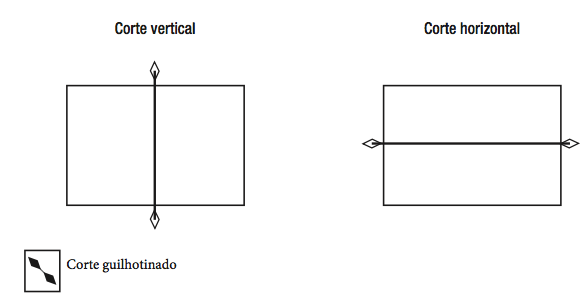
\includegraphics[width=15cm, height=5cm]{imagens/guilhotine2}
    \caption{Exemplos de cortes}
  \end{figure}
	
		Segundo  \cite{cutint} o problema para cortes em peças limitadas pelo tamanho do objeto origianal e maior, realizando apenas cortes guilhotináveis e não estagiados, esse problema também é conhecido como  Problema de Corte Bidimensional Guilhotinado e Restrito.
	

\subsection{Corte guilhotinado}
\label{sub:corte_guilhotinado}

Para gerar um corte guilhotinado utilizamos o seguinte método:

\begin{python}
    def __stupid_cut(self, x0, y0, x1, y1, pieces):
        w, h = x1 - x0, y1 - y0
        if len(pieces) > 0:
            p, *tail = pieces
            pw, ph = p
            if pw <= w and ph <= h:
                right_cuts, tail = self.__stupid_cut(x0+pw, y0, x1, y0 + ph, tail)
                above_cuts, tail = self.__stupid_cut(x0, y0+ph, x1, y1, tail)
                return ((x0, y0, pw, ph, 1, right_cuts, above_cuts), tail)
        return (None, pieces)
\end{python}

O método de corte recebe uma area retangular e uma lista de peças a serem
inseridas. Enquanto existem peças, ele seleciona a próxima peça e caso ela
caiba no espaço destinado, é inserida. Caso contrário, o espaço fica vazio e a
lista de peças é retornada.

Caso a peça seja encaixada, uma tupla com a seguinte configuração por posição é retornada:

\begin{enumerate}
    \item Tupla:
        \begin{enumerate}
            \item x0: posição inferior no eixo X onde a peça foi inserida
            \item y0: posição inferior no eixo y onde a peça foi inserida
            \item pw: largura da peça
            \item ph: altura da peça
            \item q: quantidade de peças iguais repetidas (nesse artigo o valor é sempre 1, repetições só acontecem ao acaso)
            \item right\_cuts: cortes à direita, gerados com chamada recursiva ao mesmo método
            \item above\_cuts: corte acima, geradora com chamada recursiva ao mesmo método
        \end{enumerate}
    \item pieces: lista de peças não utilizadas na chamada
\end{enumerate}

A lista de peças não utilizadas é retornada para que as chamadas recursivas subsequentes não reutilizem peças indevidamente.

\section*{Perturbação e Vizinhança}

Perturbarção é o termo utilizado para nomear o processor de modificar
sutilmente uma candidata à solução em um algoritmo que utiliza meta-heuristica.
Ao gerar uma perturbação, dizemos que a nova solução é vizinha de sua geradora.

O método que utilizamos para gerar perturbações para nossa \textit{Simulated Anealing} é o seguinte:

\begin{python}
    def change(self, pieces):
        change_index = random.randint(0, len(pieces)-1)
        new = random.choice(self.rects)
        pieces = pieces[:change_index] + [new] + pieces[change_index:]
        return self.pieces(self.cut(pieces))
\end{python}

O método acima seleciona posição para inserir uma nova peça, modificando a sequencia original em $O(1)$. Este processo é seguido pela geração de um novo corte a partir da lista de peças com esta ligeira modificação.

Durante o processo de gerar o novo corte, podemos ter resultados bem diferentes mesmo com uma modificação tão sutil:

\begin{itemize}
    \item Caso a nova peça tenha altura inferior à peça deslocada, a linha à direita desta peça ficará vazia. Isto se dá pela forma que o método gerador de corte trabalha, caso ele não consiga inserir a peça na mesma linha, ele abre uma nova linha acima, deixando espaço vago no restante da linha, caso haja;
    \item Caso a peça adicionada seja maior que sua predecessora, o citado também acontece, só que agora à partir da nova peça inserida;
    \item Existe a possibilidade de uma peça ser inserida nesses espaços vazios, uma grande quantidade de perturbações pode garantir que tal cenário ocorra;
\end{itemize}

    Como o método change só insere elementos à princípio, o seu retorno é fruto de uma formação de corte, fazendo com que peças sejam descartadas caso não haja mais espaço para a próxima peça. Depois de se determinar o corte as peças são estraídas e retornadas.

\section*{Meta-Heurística \textit{Simulated Anealing}}

De acordo com \cite{KirkSA}, a meta heuristica Simulated Annealing (S.A) é uma técnica oriunda de uma analogia com a termodinamica para obter estados de baixas energias em um sólido. Como meta heuristica, ela é utilizada em problemas de otimização de busca local com probabilidade. 
Inicialmente o S.A a busca a partir de um indice qualquer, iniciando um laço em que cada interação procura um candidato seguinte para um ponto minimo na vinzinhança do atual candidato. Essa forma é dada pela seguinte diferença entre as funções objetivas:

$ {\triangle = f (s^1) - f(s) }$

Logo se $ {\triangle < 0 }$, houve uma diminuição na função objetiva e $ s^1$ é considerava como nova solução. Caso $ {\triangle = 0 }$ ou $ {\triangle > 0 }$ houve um aumento ou estabilidade da energia e a aceitação dessa solução será feita sobre um fator estatistico onde é mais provável para autas temperaturas e menos provável para menores. O fator utilizado é conhecido como fator de Boltzmann, dado por: $ {e^{(\triangle / T)} }$ onde T é a temperatura que regula a aceitação da solução de pior custo.

Essa implementação é vista no código fonte em:

\begin{python}
        def execute(self, start):
        solution = start
        temperature = self.__initial_temperature(solution)
        success_iterator = 0
        temperatures = []
        costs = []
        solutions = []

        no_change_counter = 0
        for j in range(0, self.MAX_INTERATIONS):
            for i in range(0, self.MAX_RANDOMIZE):
                new_solution = self.__randomize(solution)
                diff_s = self.__diff_solution(new_solution, solution)

                try:
                    if diff_s >= 0 or math.exp(-diff_s / temperature) > uniform(0, 1):
                        solution = new_solution
                        success_iterator = success_iterator + 1
                        
                except:
                    pass

                if success_iterator >= self.MAX_SUCESS:  
                    break

            solutions.insert(j, self.__cost(solution))
            if j > 0 and solutions[j] == solutions[j-1]:
                no_change_counter += 1
            else:
                no_change_counter = 0

            temperatures.append(temperature)
            costs.append(self.__cost(solution))

            temperature = self.ALPHA * temperature

            if success_iterator == 0 or 0.2 * self.MAX_INTERATIONS <= no_change_counter:  # stop condition
                break

        return temperatures, costs, solution
\end{python}

A temperatura inicia com um valor alto, mas após uma quantidade fixa de interações ($MAX\_INTERATIONS$) vai gradativamente caindo em razão de um fator, ALPHA, dessa forma o algoritmo tende a escapar de ficar preso em mínimos locais. Com a aproximação da temperatura a 0, o algoritmo se comporta como método de descida, já que a probabilidade de aceitar funções que piorem é muito baixa.
O algoritmo encontra sua condição de parada se a temperatura chegar próxima a 0 ou nenhuma nova solução aceita após várias interações, ou seja, o sistema está estável.


\section*{Execução dos Testes}

\begin{center}
    \resizebox{\textwidth}{!}{%
    \begin{tabular}{ |c|c|c|c|c|c|c|c|c|}
    \hline
        \# & Instancia & \# de Itens & Tam. Placa & S. Inicial & S. Média & S. Melhor & Desperdício & Tempo (s) \\ \hline

1 & cut12 & 50 & 1000x1000 & 245443 & 26131955 & 960379 & 3.96 & 1.505860 \\ \hline
2 & cut13 & 32 & 3000x3000 & 1819609 & 33351152 & 8296226 & 7.82 & 7.122655 \\ \hline
3 & cut14 & 34 & 3000x3000 & 1160710 & 20266030 & 8443673 & 6.18 & 13.024269 \\ \hline
4 & cut17 & 82 & 3500x3500 & 3063289 & 40185532 & 11142932 & 9.04 & 8.674745 \\ \hline
5 & cut1 & 10 & 250x250 & 35358 & 1416513 & 58136 & 6.98 & 1.410658 \\ \hline
6 & cut2 & 20 & 250x250 & 26941 & 1265506 & 53357 & 14.63 & 1.742492 \\ \hline
7 & cut5 & 10 & 500x500 & 191038 & 7183387 & 219110 & 12.36 & 1.299100 \\ \hline
8 & cut7 & 30 & 500x500 & 83885 & 5937212 & 244655 & 2.14 & 1.472742 \\ \hline
9 & cut9 & 10 & 1000x1000 & 299700 & 24435095 & 953628 & 4.64 & 1.634113 \\ \hline
10 & livre & 82 & 3500x3500 & 2972333 & 25909328 & 11002738 & 10.18 & 14.329081 \\ \hline

    \end{tabular}}
\end{center}



\begin{figure}
\centering
\begin{subfigure}{.5\textwidth}
  \centering
  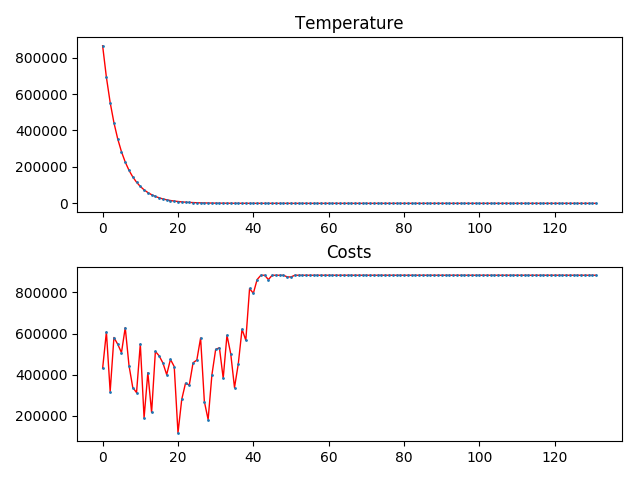
\includegraphics[width=1\linewidth]{results/cut12/3/plot}
  \label{fig:sub1}
\end{subfigure}%
\begin{subfigure}{.5\textwidth}
  \centering
  
\includegraphics[width=1\linewidth]{results/cut12/3/cut}
  \label{fig:sub2}
\end{subfigure}
\caption{Instancia cut12.txt, Solução: 975059, desperdício de 2.49\% de 1000x1000, {(599, 269): 1, (359, 728): 1, (352, 268): 1, (640, 716): 1}}
\label{fig:test}
\end{figure}


\begin{figure}
\centering
\begin{subfigure}{.5\textwidth}
  \centering
  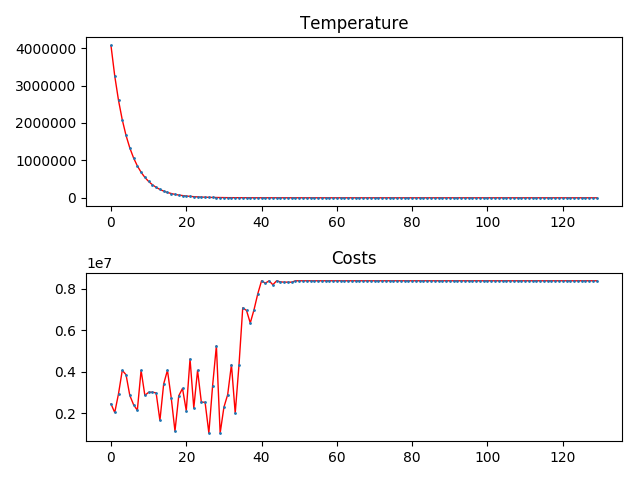
\includegraphics[width=1\linewidth]{results/cut13/1/plot}
  \label{fig:sub1}
\end{subfigure}%
\begin{subfigure}{.5\textwidth}
  \centering
  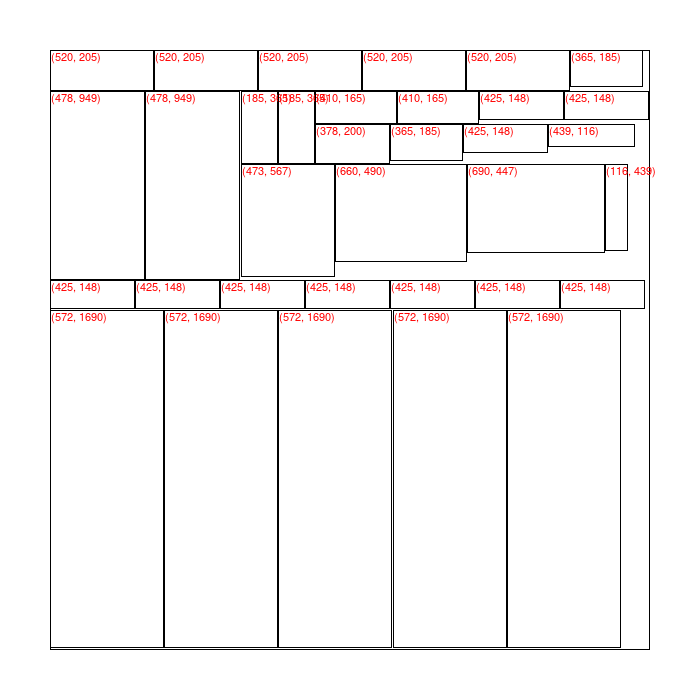
\includegraphics[width=1\linewidth]{results/cut13/1/cut}
  \label{fig:sub2}
\end{subfigure}
\caption{Instancia cut13.txt, Solução: 8212359, desperdício de 8.75\% de 3000x3000, {(540, 530): 1, (496, 555): 1, (520, 205): 1, (365, 185): 1, (116, 439): 1, (949, 445): 2, (296, 425): 1, (572, 1890): 5, (410, 165): 2, (148, 425): 1, (530, 540): 1, (205, 520): 1, (200, 378): 1, (567, 473): 1}}
\label{fig:test}
\end{figure}



\bibliography{scibib}

\bibliographystyle{Science}

\end{document}




















